\documentclass{acmsiggraph}
\usepackage{graphicx}
\usepackage{amsmath}
\usepackage{url}

\usepackage{amsmath, amsfonts}

\DeclareMathOperator{\tr}{tr}
\DeclareMathOperator{\Expect}{E}
\DeclareMathOperator{\KL}{KL}
\DeclareMathOperator{\maximize}{maximize}
\DeclareMathOperator{\subjto}{subject\quad to}
%% The 'graphicx' package allows for the inclusion of EPS figures.

\usepackage{fp}
\usepackage{graphicx}
\usepackage{color}
\definecolor{darkblue}{RGB}{19,46,82}
\definecolor{darkgreen}{RGB}{18,47,30}
\definecolor{stanford}{RGB}{164,0,29}
\usepackage{listings}
\lstset{
language=Python,
basicstyle=\sffamily,
breaklines=true,
tabsize=4,
numbers=left,
numberstyle=\small,
frame=lines,
columns=fullflexible,
showstringspaces=false,
keywordstyle=\bfseries\color{darkblue},
commentstyle=\itshape\color{darkgreen},
stringstyle=\color{stanford}
}

\begin{document}

\title{Predicate learning for probabilistic program induction}

\author{Lingfeng Yang}
\maketitle

\begin{abstract}
We present a method for augmenting Bayesian model merging-based
algorithms for probabilistic program induction
with background knowledge.
Typical model merging algorithms
do not explicitly encode relationships
between arguments (subtrees) of invented functions (non-terminals).
Furthermore, implicitly, only structural and symbolic \emph{equality} is preserved.
Given a set of atomic feature functions and an existing stochastic function,
we learn a conjunction of predicates over its arguments,
encoding a probabilistic relation.
One use of these learned predicates
is to use any discovered functional relations
between arguments to shorten the original function:
\emph{functional deargumentation}.
We demonstrate this method
for the domain of arithmetic,
evaluating its robustness to noise
on a few simple test cases.
\end{abstract}

\section{Introduction}

% Motivation for BPM + predicate learning:

Web pages, vector art, 3D models, natural language text, and other forms of structured data
may be broken down into two kinds of components:
the \emph{structure}, which describes how elements (tables, models, pictures, etc) are grouped hierarchically,
and \emph{parameters}, which describe how each element is concretely instantiated in space
(position, rotation, width, height, etc).
Previously, for automated reasoning on these forms of data,
it was popular to encode a fixed structure,
then apply a machine learning algorithm on the parameters.
Recently, structured machine learning algorithms,
which do not assume a fixed structure,
have come into wider use.
One such approach is program induction,
where the goal is to learn a computer program that generates the data.
By choosing the appropriate language from which programs are synthesized,
one can more tightly integrate the relationships between structure and parameters
into the learning process.

Previous work in program induction has 
focused on learning deterministic programs
against input with no noise.
Here, we are concerned with the induction of \emph{probabilistic} programs
over noisy input.
Unlike deterministic programs, probabilistic programs contain \emph{nondeterministic} terms;
terms that evaluate to multiple values,
and thus correspond to multiple alternate executions.
Specifically, we use a \emph{stochastic $\lambda$-calculus},
which includes a statement for probabilistic choice
in addition to the core $\lambda$-calculus
and domain-specific built-in functions.

Approaches for program induction fall along a spectrum,
where at one extreme, \emph{generate-and-test},
we exhaustively enumerate or sample complete programs
and test each one against the data.
At the other extreme, \emph{analytic},
the structure of the data
determines the structure of the program,
similar to parsing algorithms.

Here, we present an extension of \emph{Bayesian program merging},
which is an analytic probabilistic program induction method.
In this setting, the input is a set of structured data examples
$e_1, \ldots, e_n$
and the program being learned is a function $p*$ that takes no arguments.
The program is initialized to be a random draw over the input examples.
In Bayesian program merging, this initial program is iteratively refined
until an optimal balance is achieved between program size and fitting to the data.
This is formulated as an optimization of probabilities:

\begin{align*}
p* = \arg \max_{p} P(p | e_1 \ldots e_n) \propto P(e_1 \ldots e_n | p) P(p).
\end{align*}

$P(e_1 \ldots e_n | p)$ is the likelihood of the data examples and 
$P(p)$ is the prior over programs.
We use a length-based prior $P(p) = e^{-|p|}$, favoring shorter programs.

Without our extension, there are two refinement moves:
\emph{inverse inlining} and \emph{deargumentation}.
Inverse inlining takes a pair of expressions and
returns a lambda abstraction that generalizes over that pair,
inserting variables in the places the expressions are different.
For example, if the first expression was $3 + 2$ and the second expression was $3 + 4$,
inverse inlining would produce $f(x) = 3 + x$.
Deargumentation is a transformation that removes a variable from an existing abstraction,
replacing it with a random choice over its instantiations.
For example, $f(x) = 3 + x$ deargumented with respect to the applications $f(2)$ and $f(4)$
would result in $g() = 3 + choose(0.5, (2, 4))$,
where the $choose$ term denotes a stochastic choice picking $2$ or $4$ with probability $0.5$.
More details can be found in a report on Bayesian program merging\cite{}.
These moves are similar to merging 

However, these two transformations
do not take into account relations between arguments to
the invented functions and they do not use background knowledge regarding
parameters; they only use the structure.
By taking these into account,
programs can be made shorter while maintaining fit to the data.

Specifically, we investigate a new kind of program refinement that takes into account both
relations between arguments and background knowledge,
called \emph{functional deargumentation},
which replaces the argument to a function
not with a distribution or constant,
as is the case with previous deargumentation transforms,
but with a function of other arguments.
For example, for a particular function $f(x, y)$,
we find a functional relationship $g(x) = y$ between x and y
that characterizes $x$ and $y$ over the arguments 
$f$ was instantiated to.
$f(x, y)$ can then be simplified to a function of 1 argument $f'(x) = f(x, g(x))$.

Our approach is to first learn relations between arguments according to a background theory,
then use a set of rewriting rules to transform these relations into substitution equations.
These equations can then be applied to the original function
so as to minimize the number of variables the function uses.
The benefit is the same as any other deargumentation transform:
the more applications of the original function are in the program,
the greater the effect this will have on program length,
while minimally affecting fit.

To demonstrate this approach,
we use arithmetic as a background theory in our examples.
The resulting refinements are to simplify functions
so that one argument can be expressed as an arithmetic function of another:
\emph{arithmetic deargumentation}.
Using this refinement, we can achieve further compression
of programs that use numbers as parameters.
This refinement can also apply for recursive functions and in noisy settings.
We are also able to learn non-trivial compositions of basic arithmetic functions
through an iterative substitution-finding algorithm.

\section{Overview}

% TODO: overview figure
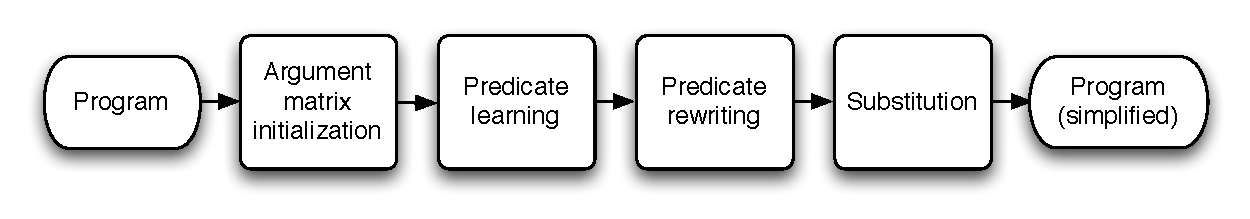
\includegraphics[width=0.48\textwidth]{figures/pipeline.pdf}

The process by which functional deargumentation transforms are created can be divided into four stages.
Given an existing program $p$ and a function on which to perform the transformation, $f$:

\begin{enumerate}
\item \emph{Initialize the argument matrices} of $f$.
The $i$-th row of the argument matrix corresponds to the arguments used in the $i$-th call to $f$,
and the $j$-th column corresponds to all instantiations of the $j$-th argument.
We also initialize the argument matrices in a way such that
if there is a call to $f$ itself as an argument,
we will order the columns of the argument matrix
according to this structural relationship.
This allows us to infer relations between arguments in \emph{nested} calls to $f$,
which is useful for simplifying recursive functions using functional deargumentation.

\item \emph{Learn predicates} between arguments to $f$. We use each row of each argument matrix
as a data example, and apply a coarse-to-fine feature induction algorithm
to find the predicates.

\item \emph{Rewrite predicates into substitutions}. The idea is that some predicates,
or combinations thereof, can encode a functional relationship among the variables involved.

\item \emph{Apply substitutions} to the original function,
with the goal of minimizing the number of used variables.
\end{enumerate}

The output is a function that is possibly simplified by using fewer variables.

\section{The argument matrix}

A convenient formalism that our method uses is the
\emph{argument matrix} corresponding to a function.
This is a matrix where each row corresponds to an application,
and the $j$-th entry of each row corresponds to the value of the $j$-th argument.
To illustrate, consider the following program, function $f$, and argument matrix:

\begin{lstlisting}
program:
(let ()
    (list (f 1 3) (f 2 4) (f 5 7))
    )

function: 
    (define (f x y) (+ x y))

argument matrix: 
[[1 3]
 [2 4]
 [5 7]]
\end{lstlisting}

In the case of nested calls to $f$,
we will create multiple argument matrices,
one corresponding to each nesting.
The columns will also be ordered according to the nesting.
For example:

\begin{lstlisting}
program:
(let ()
    (list (f 1 (f 2 (f 3 4)))
        (f 8 9)
        (f 10 (f 11 12)))
    )

function: 
    (define (f x y (cons x y)))

argument matrices: 
[[1 (f 2 (f 3 4))]
 [2 (f 3 4)]
 [3 4]]

[[8 9]]

[[10 (f 11 12)]
 [11 12]]

\end{lstlisting}

The reason for this splitting is that
we are also interested in learning functional relationships
between arguments of the same name,
but at different levels of recursion.

\section{Learning conjunctions of features}

After we obtain the argument matrix, the next step is to learn predicates.
We map the argument matrix to a set of data examples.
If we wish to capture relationships between arguments,
we map each row to a data example.
Otherwise, if we are interested in the relationship
between calls to the function for the same argument at different levels of recursion,
we map each pair of consecutive values in the column to a data example.

Then, given a set of $n$ data examples (which can be a set of rows or consecutive columns),
each of which is a vector of length $k$:

\newcommand{\EX}[1]{{\mathbf{x}^{(#1)}}}

\begin{align*}
\EX{1}, \EX{2}, \ldots \EX{n},
\end{align*}

we learn a conjunction of atomic background knowledge features that best fits this data.
This can be seen as a program induction subroutine in the larger probabilistic program induction algorithm,
where the language is conjunctions of atomic features.
It also receives a probabilistic treatment:

\begin{align*}
p* &= \arg \max_p \prod^n_{i = 1} P(p | \EX{1}, \ldots, \EX{n}) \propto \\
&P(\EX{1}, \ldots, \EX{n} | p) P(p),\\
p(x_1, x_2, \ldots x_k) &= p_1(x_{11}, x_{12}, \ldots) \wedge p_2(x_{21}, x_{22}, \ldots),
\end{align*}

We use the following formulas for the likelihood and prior:

\begin{align*}
P(\EX{1}, \ldots, \EX{n} | p) &= \prod^n_{p_i \in p} p_i(\{x_i\}),
P(p) &= \alpha e^{|p|}.
\end{align*}

The likelihood is the product of all feature functions.
In the case of hard predicates (those returning only 0 or 1), 
it acts like \emph{logical} conjunction.
The prior favors long predicates; i.e., the more facts we can show about the example, the better.
Thus, the optimal predicate balances fitting the data with being as descriptive as possible.
Note that this contrasts with the prior for the overall program,
which favors \emph{shorter} programs.
A natural extension to this is to explore more informative priors,
such as favoring predicates that are logically consistent
according to the background theory.

\subsection{Encoding background knowledge}

Throughout this paper,
we use arithmetic as an example of the background knowlege
we are interested in incorporating.
It is composed of the following binary atomic feature functions:

\newcommand{\Equals}{\textup{Equals}}
\newcommand{\Offby}{\textup{Offby}}
\newcommand{\Greater}{\textup{Greater}}
\newcommand{\Neg}{\textup{Neg}}
\newcommand{\Ratio}{\textup{Ratio}}
\newcommand{\AND}{\wedge}

\newcommand{\Gauss}[3]{N_{#1}(#2, #3)}
\newcommand{\Sigmoid}[3]{\frac{1}{1 + e^{-(#2 - #1) #3}}}

\begin{align*}
\Equals(x, y) &= \Gauss{|x - y|}{0}{0.1} \\
\Greater(x, y) &= \Sigmoid{x}{y}{10} \\
\Offby(n, x, y) &= \Gauss{|x - y|}{n}{0.1} \\
\Ratio(n, x, y) &= \Gauss{x / y}{n}{0.1} \\
\Neg(x, y) &= \Ratio(-1, x, y).
\end{align*}

where $\Gauss{x}{\mu}{\sigma^2}$ is the Gaussian pdf with domain $x$, mean $\mu$ and variance $\sigma^2$.
We use $\Neg(x, y)$ because it results in a slightly more simplified substitution equation ($x = -y$)
than with $\Ratio(-1, x, y)$ ($x = -1 * y$).
In the long term, however,
it would be proper to more cleanly separate
the simplification of expressions
from finding the relations between arguments.

\subsection{General-to-specific feature induction.}

We use general-to-specific search over conjunctions of atomic features to find $p*$.
This is inspired by (probabilistic) inductive logic programming (PILP).
In general-to-specific search, we start with an empty conjunction that does not
favor any set of data points over any other, and iteratively add a feature to
the conjunction that maximizes the posterior probability of the entire conjunction.
The result is a predicate that is just barely general enough to fit all examples.
The rationale behind general-to-specific search comes from the monotonic behavior of conjuctions;
that more points will evaluate to true, or get a higher raw score, under $p_1
\wedge \ldots \wedge p_n$ than $p_1 \wedge \ldots \wedge p_n \wedge p_{n + 1}$.

However, there are crucial differences from learning from interpretations in PILP.
First, for noisy floating-point data, we perform this over \emph{soft} features,
not to be confused with the \emph{noisy} features used in PILP.
This causes certain problems. For one thing, one cannot use normal unification
to find the maximizing parameters in parameterized predicates.
Instead, one has to perform a 'soft' version of unification.
Second, we do not learn complete (probabilistic) Prolog programs;
we only learn one Horn clause,
with each conjunction being a linear term (no repeated variables)
and no local variables.

\lstset{language=LISP}
\lstinputlisting[caption=The feature induction algorithm.]{feature_induction.ss}

\paragraph{Soft unification.}

With non-parameterized predicates
such as $\Equals(x, y)$,
we can calculate the likelihood of the data example
given a hypothesis with $\Equals(x, y)$ immediately.
However, when working with parameterized predicates
such as $\Offby(n, x, y)$, there is actually a two-step process
in calculating the likelihood of a particular refinement
that uses them. 
Normally, in the probabilistic inductive logic setting,
unification would be used to find the parameter that would fit the data.
However, in our setting we are dealing with \emph{soft}
feature functions on \emph{noisy} data;
unification as we know it breaks down.
Instead we use \emph{soft unification};
finding a parameter $n$ that would maximally fit
the feature (or, in general, the entire hypothesis) to the data.
Currently, we calculate the optimal parameter
for each data example, then take the sample average of these parameters
and use that in the likelihood calculation.
This works for arithmetic predicates,
but in general we would need to run some optimization algorithm
to find these parameters.

\section{Simplifying the function by substituting variables}

Given a conjunction of predicates learned from data,
it is possible that they impose \emph{functional} relations between variables.
For example, suppose $x > y \wedge |x - y| = 1$; then $y = x + 1$.
In general, we can \emph{specialize} a function
to the data examples according to some theory (in this case, arithmetic).
We perform this in three stages: 
rewriting the predicates into substitution equations,
finding equivalence classes corresponding to the equations,
and deriving a set of substitutions according to the equivalence classes and equations
that minimizes the number of variables used.

\paragraph{Rewriting predicates into substitution equations.}
We specify a set of \emph{rewriting rules}
that take a conjunction of predicates to a set of \emph{substitution equations}
that relate one variable in terms of a function application of another variable:


\begin{align*}
x = y &\leftarrow \Equals(x, y) \\
x = -y &\leftarrow \Neg(x, y) \\
x = y + n &\leftarrow \Offby(n, x, y) \AND \Greater(x, y) \\
x = y + n &\leftarrow \Offby(n, y, x) \AND \Greater(x, y) \\
x = y * n &\leftarrow \Ratio(n, y, x) \AND \Greater(x, y) \\
x = y * n &\leftarrow \Ratio(n, x, y) \AND \Greater(x, y)
\end{align*}

Applying all rewriting rules to a set of predicates
yields a corresponding set of substitution equations.
For example, the substitution equations corresponding to the predicates

\begin{align*}
\Neg(x_1, x_2) \AND \Offby(1, x_1, x_3) \AND \Greater(x_3, x_1) \AND \Neg(x_3, x_4)
\end{align*}

are

\begin{align*}
x_1 &= -x_2 \\
x_3 &= x_1 + 1 \\
x_4 &= -x_3.
\end{align*}

One can think of the rewriting rules
as a separate query that discovers further relations
according to a background knowledge theory.

\paragraph{Finding equivalence classes} The next phase concerns
restricting and organizing the space of possible substitutions.
We do this by finding equivalence classes of patterns
that occur in each substitution equation;
i.e., which patterns can be freely substituted for another
without changing the semantics of the program.
We view the substitution equations as specifying a graph,
where each vertex is a pattern and each edge
connects two vertices if the corresponding patterns are related by $=$.
The equivalence classes of interest are then the connected components of this graph,
including the original variables.
For example, the equivalence classes corresponding to the previous example are

\begin{align*}
\{x_1\}, \{x_3, x_1 + 1\}, \{x_4, -x_3\}, \{x_2, -x_1\}.
\end{align*}

Recall that our goal is to
substitute patterns in the original function
so that it can be expressed with fewer variables.
Note that this cannot be accomplished simply by,
say, substituting patterns in each equivalence class
with the representatives that use the least number of variables.
For the classes above, they would be
$x_1, x_1 + 1, -x_3$ and $-x_1$ respectively, but
we know that $x_4= -(x_1 + 1)$;
a better set would be $x_1, x_1 + 1, -(x_1 + 1)$ and $-x_1$,
which would only use one variable.
The problem is finding \emph{compositions} of substitutions
that result in representatives with the fewest number of variables.

To address this, our algorithm \emph{interleaves} substitution application with representative finding.
We iteratively choose the representative patterns the \emph{most common variable}
(given the representatives chosen so far),
possibly leaving some remaining classes without representatives,
and apply the resulting substitutions to the remaining classes.
In this case, we would first pick the following representatives and leave the following classes
(because $x_1$ is the most common variable):

\begin{align*}
\{x_1\} &\rightarrow x_1 \\
\{x_3, x_1 + 1\} &\rightarrow x_1 + 1 \\
\{x_4, -x_3\} &\rightarrow \emptyset \\
\{x_2, -x_1\} &\rightarrow -x_1.
\end{align*}

Now we have representatives for substituting $x_3,$ and $x_2$
that only use $x_1$: $x_1 + 1$ and $-x_1$, respectively.
We then do so in the remaining pattern: $\{x_4, -x_3\} \rightarrow \{x_4, -(x_1 + 1)\}$.
Then we, at the next iteration,
find a representative for that pattern
that uses the most common variable: $-(x_1 + 1)$.
We obtain the optimal set of representatives
as a result,
and the function may be written in terms of one argument only.

Here is a sketch of the substitution-finding algorithm.
We iteratively find the most common variable that occurs
in the set of representatives and classes,
pick representatives in the remaining equivalence classes
according to it,
and apply the resulting substitutions to the classes left over.
\lstinputlisting[caption=Finding the best representatives by interleaving substitutions.]{substitutions.ss}

However, this algorithm's correctness depends on the form of substitution equations learned.
This is because the interleaved subsitutions
are unidirectional; a variable is always being replaced by a pattern,
and not the other way around.
In particular,
for the previous example, 
we would not have obtained a set of representatives in one variable
if we had the classes $\{x_1, -x_2\}$ and $\{x_2\}$
instead of $\{x_1\}$ and $\{x_2, -x_1\}$;
in this case, we would never have found $-x_1$
as the representative for $\{x_2\}$, as $\{x_2\}$
does not occur by itself in any other class,
then there would not have been an intervening substitution
that would have revealed it.
This suggests learning several equations expressing the same relation,
each one formulating it where the variable is 'solved' for 
i.e., generating both $x_1 = -x_2$ and $x_2 = -x_1$ from $\Neg(x_1, x_2)$,
and both $x_3 = x_1 + 1$ and $x_1 = x_3 - 1$ from $\Offby(1, x_1, x_3) \AND \Greater(x_3, x_1)$.

\section{Results}

We demonstrate the arithmetic deargumentation transform
on data of varying amounts of noise.
We generate each set of data examples
according to a 'ground truth' model
that is based on noisy addition and multiplication,
which work by adding or multiplying by the respective identity element (0 or 1)
perturbed by a sample from a Gaussian centered at zero
with variance a parameter.
We can then evaluate the arithmetic deargumentation transform
by how robust it is to noise
through testing the same model
at different amounts of variance,
where zero variance corresponds to non-noisy data.
We find that the algorithm degrades in a safe direction;
if the data is too noisy,
no deargumentation will be performed.

\lstinputlisting[caption=Results on data of increasing noise]{concept-tests.scm}

Note that for some concepts,
the algorithm degrades much more quickly
than others.
This may be avoided
if we also optimized the parameters
for each soft atomic feature.
Future work would involve 
combining techniques in structured machine learning
to handle these continuous cases.

% \section{Discussion}
% 
% % Need to try more background domains and such
% 
% While we only show results for arithmetic deargumentation,
% this method method can apply to other domains as well.
% We already have a framework for constructing other deargumentation moves of this type.
% The user provides a set of background predicates
% along with rewriting rules that
% send a set of predicates to a set of substitution equations.
% Our system will transform the learned predicates into substitution equations
% and apply the substitutions in a greedy manner so as to
% minimize the number of variables used.
% It would be interesting to see how this approach could inform the design of a general framework for 
% designing a probabilistic program induction algorithm
% for a particular domain.
% 
% % Factor pieces out into separate systems: 
% 
% % 1. the algebraic datatype
% 
% % 2. the program scheme (uniform-draw or whatever)
% 
% % 3. refinements of the program
% 
% % 4. domain-specific background knowledge (PILP)
% 
% % Possible applications
% 
\end{document}

